\documentclass{jsarticle}
\usepackage{amsmath}
\usepackage[dvipdfmx]{graphicx}
\usepackage[dvipdfmx]{color}
\usepackage{float}
\begin{document}
\title{修論進捗メモ}
\author{萱場 悠貴}
\maketitle

\section{2018/11/16発表}
\subsection{修正部分など}
\begin{itemize} %点を打つ%
\item 分析対象を拡張

分析対象を東京、大阪、福岡の3都市から東京、大阪、福岡、札幌、那覇の5都市に拡張した。

これは反実仮想シミュレーションにおいて北海道新幹線開通の影響を見るためである。

\item 運賃パラメータの符号

関数Objectiveで運賃パラメータの正負が入れ替わっているというミスを発見したので修正した。

このミスの発見により、正しく最適化できていたということが示唆されたがその一方で効用関数推定において運賃パラメータが正になっていることが重荷としてのしかかってくるようになった笑

\item JR部分の需要

シミュレーション結果において、鉄道経路の選択確率は実績値と乖離するようにプログラムが組まれているが、需要量については実績値のまま表示されているのでそこは修正する必要がある。

\item JR部分の運賃

シミュレーションを実行してsimulationresults.csvが生成されるわけだが、それが生成される前にJRの運賃を2倍する必要がある。航空運賃が往復運賃、JRが片道運賃で入っていたところを半分にしてからシミュレーション行っているのでこの処置が必要となる。
現状では別途組んだエクセルのマクロで対処されているが、それだとグラフを描くときに2倍が反映されないのでその前の段階で修正する。

\item 運賃の2次の項

前回の発表で運賃の項を2次で入れて上に凸の形で表現するのはどうかというアドバイスがあったが、Supply Analysis 4のほうもそれに合わせた修正が必要になる。
具体的には、効用関数が9つの項からなるのでそれを変更するのと、関数Objectiveなどにもそれを反映させる必要があるということに留意する必要がある。

→反映させた。やはり暴走する(均衡運賃は7万円台、二次関数のピークは67875)

\end{itemize}

\subsection{反実仮想シミュレーションについて考える}

ここから反実仮想シミュレーションについて考える。ポイントをつらつらと書く。

\begin{itemize} %点を打つ%
\item シミュレーション対象

とりあえず北海道新幹線札幌開業を考える。他の候補は新幹線延伸、LCCの参入くらいしか思いついていないのでなんか考えなければ。経済厚生の変化とかに落とせたりしないかな。

\item 用意すべきもの
\begin{itemize}
\item 仮想の所要時間、運賃、滞在可能時間、アクセシビリティ(これは現実のをぶち込めば良し)

所要時間は東京-札幌間で5時間14分、指定席特急券が東京-札幌で8090円、運賃が12910円である。滞在可能時間は24時間-(5時間14分)×2=13時間32分とする

\item 需要をどんな感じで代替するか(ODはfix、それとも何らかの方法で増やす?)
\end{itemize}
\end{itemize}

\subsection{中間報告を受けて}

とりあえず新たに出てきた課題とか先生からのアドバイスとか。

\begin{itemize} %点を打つ%
\item 課題はやはり運賃パラメータの符号条件

運賃パラメータの符号を負に差し替えれば基本的にBase Case、Counterfactualともにシミュレーションはうまくいっているのでどうにかして効用関数推定で運賃パラメータを負に出す必要がある。

考えられる方策として、

\begin{itemize}
\item 現在採用している変数を除く、あるいは新たな変数を採用する

これが一番やりやすそうではある。ただデータの収集が結構大変だし、仮に効用を運賃に単回帰したところで負に出るかどうかわからんから確かめるならまずそこからという感じはある。

\item それでいて尚且つ符号制約をかける

先々週に符号制約をかけたときは0に飛んで行ってしまったが、変数選択等を変えれば負の領域で収まる可能性はある。

\item 線形確率モデルを採用する

これよくわからんし先生もうまくいかなそうって言ってたからあまりやる意味はなさそう

\item ロジットモデルをやめる

入れ子ロジットとかランダム係数ロジットに変更すれば論文としてはより高度になるみたいなとこはある。ただ時間かけてやった挙句正負が反転しないということは十分にありえてしまうのでリスキーかなあ。もう一年あればやってもよかったけど、、、

\end{itemize}

ぶっちゃけここまで来たら気合いしかないのでゴリゴリやるしかないですね。

\item データの追加

北海道新幹線延伸開業で反実仮想をやったわけだけど東京札幌間ですら割と距離があるのであまりシミュレーションのうまみが感じられなかった。
そこで東京札幌間の各都市(仙台、青森など)をシミュレーションに含めることが検討されるわけだが、一地点追加するだけで結構大変ということが発覚したのでこれはやるなら早めに動いたほうがよさそう。
アクチュアリー試験あるからあんま修論やってる場合ではないんだがなあ、、

\end{itemize}

取りあえずパッと思いつくのはこのくらい。1.1節に書いたこともまだ治ってなかったりなのでそれはちゃんとやったほうが良い。


\section{2018/11/21発表}
\subsection{修正進め方}

もはや符号条件に合致した効用関数パラメータを得るしかない状況なので、いろいろ頑張っていきたい。その前に、どんな変数が入っていてどのような形でデータが採られているかをまず整理したい。

\begin{itemize}
\item 所要時間

航空、鉄道経路のそれぞれの所要時間(分)。航空に関しては、JTB時刻表から代表てきそうな所要時間をとってきている。エアラインごとに丸めているが、エアラインごとに所要時間は変わっていないので特にその部分で問題はなさそう。
ただ効用関数推定においては東京エリアは成田空港、大阪エリアは関西空港というように大都市圏は代表空港を定めてしまっているのでその部分は確か単純平均をとっていたような気がする。航空便数を反映して加重平均をとったほうが良いかも。
鉄道の方はよくわからんサイトからとってきた標準的な所要時間を入れているのであまり、というか本当に良くない。ただ割と所要時間に関しては大嘘というわけではく、いくつか実際の時刻表と照合してもだいたい同じだったのでいったん問題はないかと。

\item 費用

航空の方は所要時間と同じ方法で処理している。すなわちエアラインごとに異なる運賃を単純平均して算出している。問題の根幹はここなので修正すべきであろう。少なくとも航空便数で加重平均をとるくらいのことはしたほうがよさそう。
鉄道の方はもっとひどくて、駅間距離を測定し、その距離によって普通運賃を計算し、そんでそれを2倍している笑(笑い事ではない)。というわけでここは絶対に修正しなければならないのだが、どうやって修正すべきかはちょっとまだ見えていない。
最悪の場合ひと駅ひと駅運賃を計算しないといけないかもしれない。

\item 航空便数の対数

航空便数は丸める部分は総和するより外に仕方がないのでいったんオッケーといえる。ただ、年間の航空便数を入れたいがために単純に365倍しているのをどうすべきかは考えなくてはならない。あとそのせいで鉄道の方の航空便数が365本になってしまっている
問題を解決しないといけない。

\item 滞在可能時間

航空の方はちゃんとデータをとってるのでこれは良さそう。でも鉄道のほうは始発が6時、終電の到着が24時とし、そこから所要時間の2倍を引いてるので割とカスである。これも調べるの大変なのでどうしようか、、という感じである

\item アクセシビリティ指標

これを距離で妥協するのは仕方ないとして、イグレスの方のアクセシビリティを入れていないのは問題といえる。修正しよう。

\item 鉄道ダミー

これはさすがに大丈夫。

\item エアライン参入数

これどうやったか忘れたけどちゃんとやってた気がするのでいったん大丈夫でしょう。

\end{itemize}

こうしてみるとなかなかにひどい状況なので修正大変そう。頑張って4時くらいには帰るようにしたい。

\section{2018/11/30発表}

\subsection{運賃パラメータ問題についての検討}

運賃パラメータが正に出る問題についていろいろ考える。

まず運賃と選択確率の関係を可視化する。グラフは以下:

\begin{figure}[htbp]
 \begin{minipage}{0.5\hsize}
  \begin{center}
   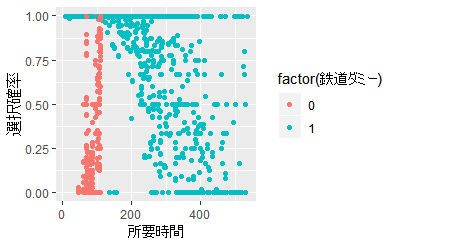
\includegraphics[width=60mm]{所要時間と選択確率.png}
  \end{center}
  \caption{所要時間と選択確率}
  \label{fig:one}
 \end{minipage}
 \begin{minipage}{0.5\hsize}
 \begin{center}
  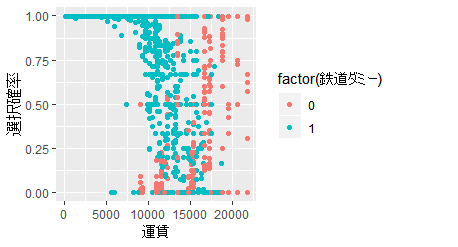
\includegraphics[width=60mm]{運賃と選択確率.png}
 \end{center}
  \caption{運賃と選択確率}
  \label{fig:two}
 \end{minipage}
\end{figure}

\begin{figure}[htbp]
 \begin{minipage}{0.5\hsize}
  \begin{center}
   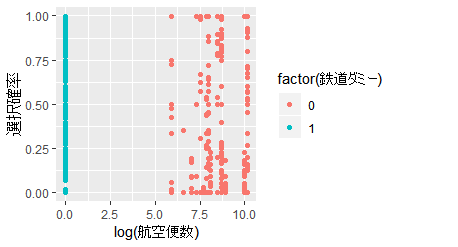
\includegraphics[width=60mm]{log(航空便数)と選択確率.png}
  \end{center}
  \caption{log(航空便数)と選択確率}
  \label{fig:three}
 \end{minipage}
 \begin{minipage}{0.5\hsize}
 \begin{center}
  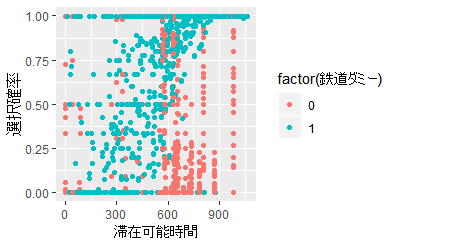
\includegraphics[width=60mm]{あああ.png} %%滞在可能時間と選択確率.png
 \end{center}
  \caption{滞在可能時間と選択確率}
  \label{fig:four}
 \end{minipage}
\end{figure}

\begin{figure}[htbp]
 \begin{minipage}{0.5\hsize}
  \begin{center}
   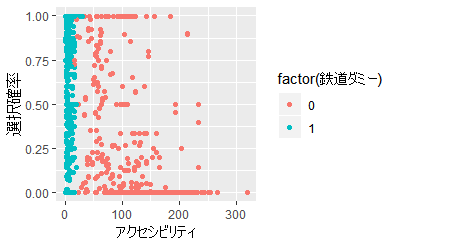
\includegraphics[width=60mm]{アクセシビリティと選択確率.png}
  \end{center}
  \caption{アクセシビリティと選択確率}
  \label{fig:five}
 \end{minipage}
 \begin{minipage}{0.5\hsize}
 \begin{center}
  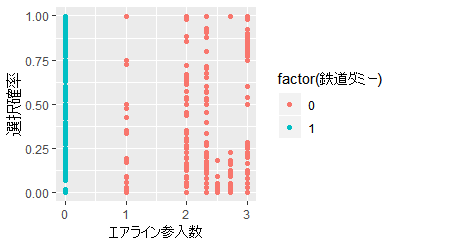
\includegraphics[width=60mm]{エアライン参入数と選択確率.png}
 \end{center}
  \caption{エアライン参入数と選択確率}
  \label{fig:six}
 \end{minipage}
\end{figure}



















図\ref{fig:one}をみると、運賃と選択確率は正の相関を持つことが示唆される。この原因として以下が考えられる。







\begin{itemize} %点を打つ%

\item 近距離においては自動車の選択確率が高い

本論文ではOD間の移動需要のうち、航空と鉄道の選択確率の実績値を求めている。残りの交通手段に関しては、いわばoutside optionという扱いにしている。
この場合、比較的近距離の移動に関しては航空便が供給されていないことが多い。また鉄道に関しても選択確率が低く、自動車を含めたoutside optionの選択確率が高くなってしまっていることが示唆される。



\end{itemize}

相関をみる

\begin{figure}[htbp]
\begin{center}
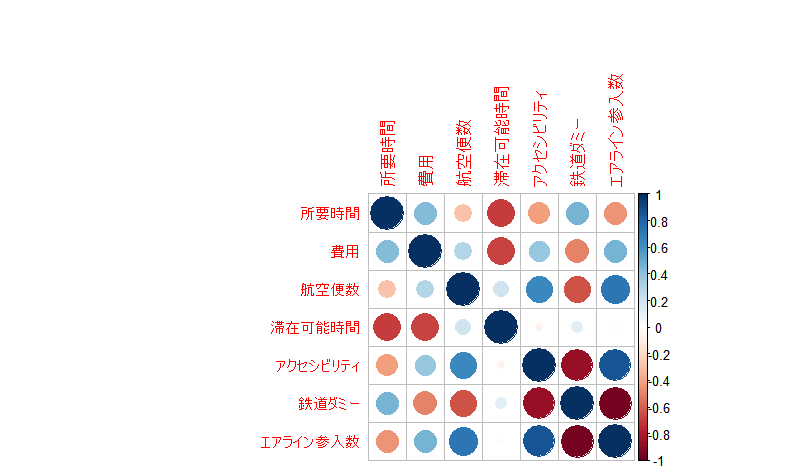
\includegraphics[width=150mm]{correlation_matrix.png}
\end{center}
\caption{相関行列}
\label{fig:seven}
\end{figure}

% latex table generated in R 3.5.1 by xtable 1.8-3 package
% Fri Nov 30 06:28:45 2018
\begin{table}[ht]
\centering
\begin{tabular}{rlllllll}
  \hline
 & 所要時間 & 費用 & 航空便数 & 滞在可能時間 & アクセシビリティ & 鉄道ダミー & エアライン参入数 \\ 
  \hline
所要時間 & 1.000 & 0.439 & -0.287 & -0.691 & -0.412 & 0.469 & -0.442 \\ 
  費用 & 0.439 & 1.000 & 0.291 & -0.679 & 0.382 & -0.491 & 0.469 \\ 
  航空便数 & -0.287 & 0.291 & 1.000 & 0.209 & 0.642 & -0.631 & 0.730 \\ 
  滞在可能時間 & -0.691 & -0.679 & 0.209 & 1.000 & -0.061 & 0.124 & -0.018 \\ 
  アクセシビリティ & -0.412 & 0.382 & 0.642 & -0.061 & 1.000 & -0.866 & 0.858 \\ 
  鉄道ダミー & 0.469 & -0.491 & -0.631 & 0.124 & -0.866 & 1.000 & -0.953 \\ 
  エアライン参入数 & -0.442 & 0.469 & 0.730 & -0.018 & 0.858 & -0.953 & 1.000 \\ 
   \hline
\end{tabular}
\end{table}












% Table created by stargazer v.5.2.2 by Marek Hlavac, Harvard University. E-mail: hlavac at fas.harvard.edu
% Date and time: 金, 11 30, 2018 - 5:48:13
\begin{table}[!htbp] \centering 
  \caption{} 
  \label{} 
\begin{tabular}{@{\extracolsep{5pt}}lcccccc} 
\\[-1.8ex]\hline 
\hline \\[-1.8ex] 
 & \multicolumn{6}{c}{\textit{Dependent variable:}} \\ 
\cline{2-7} 
\\[-1.8ex] & \multicolumn{6}{c}{y} \\ 
\\[-1.8ex] & (1) & (2) & (3) & (4) & (5) & (6)\\ 
\hline \\[-1.8ex] 
 費用 & $-$0.0004$^{***}$ & 0.0001$^{***}$ & 0.0001$^{**}$ & $-$0.0004$^{***}$ & $-$0.0004$^{***}$ & $-$0.0004$^{***}$ \\ 
  & (0.00002) & (0.00003) & (0.00003) & (0.00002) & (0.00002) & (0.00002) \\ 
  log(航空便数) & $-$0.649$^{***}$ & $-$1.308$^{***}$ & $-$0.890$^{***}$ & $-$0.093$^{**}$ & 0.234$^{*}$ & $-$1.351$^{***}$ \\ 
  & (0.024) & (0.044) & (0.025) & (0.044) & (0.121) & (0.106) \\ 
  所要時間 &  & $-$0.023$^{***}$ &  &  &  &  \\ 
  &  & (0.001) &  &  &  &  \\ 
  滞在可能時間 &  &  & 0.010$^{***}$ &  &  &  \\ 
  &  &  & (0.0004) &  &  &  \\ 
  アクセシビリティ &  &  &  & $-$0.041$^{***}$ &  &  \\ 
  &  &  &  & (0.003) &  &  \\ 
  鉄道ダミー &  &  &  &  & 7.673$^{***}$ &  \\ 
  &  &  &  &  & (1.035) &  \\ 
  エアライン参入数 &  &  &  &  &  & 2.643$^{***}$ \\ 
  &  &  &  &  &  & (0.387) \\ 
  Constant & 7.636$^{***}$ & 8.177$^{***}$ & $-$2.517$^{***}$ & 8.169$^{***}$ & $-$0.093 & 7.622$^{***}$ \\ 
  & (0.183) & (0.176) & (0.488) & (0.180) & (1.058) & (0.182) \\ 
 \hline \\[-1.8ex] 
Observations & 2,588 & 2,588 & 2,588 & 2,588 & 2,588 & 2,588 \\ 
R$^{2}$ & 0.455 & 0.514 & 0.542 & 0.498 & 0.467 & 0.465 \\ 
Adjusted R$^{2}$ & 0.455 & 0.514 & 0.542 & 0.497 & 0.466 & 0.464 \\ 
\hline 
\hline \\[-1.8ex] 
\textit{Note:}  & \multicolumn{6}{r}{$^{*}$p$<$0.1; $^{**}$p$<$0.05; $^{***}$p$<$0.01} \\ 
\end{tabular} 
\end{table}








% Table created by stargazer v.5.2.2 by Marek Hlavac, Harvard University. E-mail: hlavac at fas.harvard.edu
% Date and time: 金, 11 30, 2018 - 5:50:45
\begin{table}[!htbp] \centering 
  \caption{} 
  \label{} 
\begin{tabular}{@{\extracolsep{5pt}}lcccccc} 
\\[-1.8ex]\hline 
\hline \\[-1.8ex] 
 & \multicolumn{6}{c}{\textit{Dependent variable:}} \\ 
\cline{2-7} 
\\[-1.8ex] & \multicolumn{6}{c}{y} \\ 
\\[-1.8ex] & (1) & (2) & (3) & (4) & (5) & (6)\\ 
\hline \\[-1.8ex] 
 費用 & $-$0.0004$^{***}$ & 0.0001$^{***}$ & 0.0002$^{***}$ & 0.0002$^{***}$ & 0.0002$^{***}$ & 0.0002$^{***}$ \\ 
  & (0.00002) & (0.00003) & (0.00003) & (0.00003) & (0.00004) & (0.00004) \\ 
  log(航空便数) & $-$0.649$^{***}$ & $-$1.308$^{***}$ & $-$1.203$^{***}$ & $-$0.751$^{***}$ & 0.247 & $-$0.742$^{**}$ \\ 
  & (0.024) & (0.044) & (0.042) & (0.056) & (0.263) & (0.310) \\ 
  所要時間 &  & $-$0.023$^{***}$ & $-$0.013$^{***}$ & $-$0.012$^{***}$ & $-$0.024$^{***}$ & $-$0.021$^{***}$ \\ 
  &  & (0.001) & (0.001) & (0.001) & (0.003) & (0.003) \\ 
  滞在可能時間 &  &  & 0.008$^{***}$ & 0.007$^{***}$ & 0.002$^{*}$ & 0.003$^{**}$ \\ 
  &  &  & (0.0005) & (0.0005) & (0.001) & (0.001) \\ 
  アクセシビリティ &  &  &  & $-$0.031$^{***}$ & $-$0.031$^{***}$ & $-$0.031$^{***}$ \\ 
  &  &  &  & (0.003) & (0.003) & (0.003) \\ 
  鉄道ダミー &  &  &  &  & 10.413$^{***}$ & 6.421$^{**}$ \\ 
  &  &  &  &  & (2.680) & (2.745) \\ 
  エアライン参入数 &  &  &  &  &  & 2.179$^{***}$ \\ 
  &  &  &  &  &  & (0.366) \\ 
  Constant & 7.636$^{***}$ & 8.177$^{***}$ & $-$0.068 & 1.195$^{**}$ & $-$4.130$^{***}$ & $-$1.223 \\ 
  & (0.183) & (0.176) & (0.551) & (0.547) & (1.475) & (1.545) \\ 
 \hline \\[-1.8ex] 
Observations & 2,588 & 2,588 & 2,588 & 2,588 & 2,588 & 2,588 \\ 
R$^{2}$ & 0.455 & 0.514 & 0.556 & 0.580 & 0.582 & 0.588 \\ 
Adjusted R$^{2}$ & 0.455 & 0.514 & 0.556 & 0.579 & 0.581 & 0.587 \\ 
\hline 
\hline \\[-1.8ex] 
\textit{Note:}  & \multicolumn{6}{r}{$^{*}$p$<$0.1; $^{**}$p$<$0.05; $^{***}$p$<$0.01} \\ 
\end{tabular} 
\end{table}




% Table created by stargazer v.5.2.2 by Marek Hlavac, Harvard University. E-mail: hlavac at fas.harvard.edu
% Date and time: 金, 11 30, 2018 - 5:05:24
\begin{table}[!htbp] \centering 
  \caption{} 
  \label{} 
\begin{tabular}{@{\extracolsep{5pt}}lcccc} 
\\[-1.8ex]\hline 
\hline \\[-1.8ex] 
 & \multicolumn{4}{c}{\textit{Dependent variable:}} \\ 
\cline{2-5} 
\\[-1.8ex] & \multicolumn{4}{c}{y} \\ 
\\[-1.8ex] & (1) & (2) & (3) & (4)\\ 
\hline \\[-1.8ex] 
 費用 & 0.0001$^{**}$ & $-$0.00000 & 0.0001$^{***}$ & 0.0001$^{***}$ \\ 
  & (0.00003) & (0.00003) & (0.00003) & (0.00003) \\ 
  log(航空便数) & $-$0.890$^{***}$ & $-$0.441$^{***}$ & $-$1.349$^{***}$ & $-$2.292$^{***}$ \\ 
  & (0.025) & (0.045) & (0.149) & (0.203) \\ 
  滞在可能時間 & 0.010$^{***}$ & 0.009$^{***}$ & 0.011$^{***}$ & 0.011$^{***}$ \\ 
  & (0.0004) & (0.0004) & (0.001) & (0.001) \\ 
  アクセシビリティ &  & $-$0.031$^{***}$ & $-$0.031$^{***}$ & $-$0.031$^{***}$ \\ 
  &  & (0.003) & (0.003) & (0.003) \\ 
  鉄道ダミー &  &  & $-$7.368$^{***}$ & $-$9.890$^{***}$ \\ 
  &  &  & (1.159) & (1.208) \\ 
  エアライン参入数 &  &  &  & 2.475$^{***}$ \\ 
  &  &  &  & (0.366) \\ 
  Constant & $-$2.517$^{***}$ & $-$1.134$^{**}$ & 4.146$^{***}$ & 6.512$^{***}$ \\ 
  & (0.488) & (0.488) & (0.961) & (1.015) \\ 
 \hline \\[-1.8ex] 
Observations & 2,588 & 2,588 & 2,588 & 2,588 \\ 
R$^{2}$ & 0.542 & 0.567 & 0.573 & 0.581 \\ 
Adjusted R$^{2}$ & 0.542 & 0.566 & 0.572 & 0.580 \\ 
\hline 
\hline \\[-1.8ex] 
\textit{Note:}  & \multicolumn{4}{r}{$^{*}$p$<$0.1; $^{**}$p$<$0.05; $^{***}$p$<$0.01} \\ 
\end{tabular} 
\end{table}

% Table created by stargazer v.5.2.2 by Marek Hlavac, Harvard University. E-mail: hlavac at fas.harvard.edu
% Date and time: 金, 11 30, 2018 - 5:14:45
\begin{table}[!htbp] \centering 
  \caption{} 
  \label{} 
\begin{tabular}{@{\extracolsep{5pt}}lccc} 
\\[-1.8ex]\hline 
\hline \\[-1.8ex] 
 & \multicolumn{3}{c}{\textit{Dependent variable:}} \\ 
\cline{2-4} 
\\[-1.8ex] & \multicolumn{3}{c}{y} \\ 
\\[-1.8ex] & (1) & (2) & (3)\\ 
\hline \\[-1.8ex] 
 費用 & $-$0.0004$^{***}$ & $-$0.0004$^{***}$ & $-$0.0004$^{***}$ \\ 
  & (0.00002) & (0.00002) & (0.00002) \\ 
  log(航空便数) & $-$0.093$^{**}$ & 0.649$^{***}$ & $-$0.139 \\ 
  & (0.044) & (0.120) & (0.188) \\ 
  アクセシビリティ & $-$0.041$^{***}$ & $-$0.039$^{***}$ & $-$0.040$^{***}$ \\ 
  & (0.003) & (0.003) & (0.003) \\ 
  鉄道ダミー &  & 6.608$^{***}$ & 4.615$^{***}$ \\ 
  &  & (0.999) & (1.060) \\ 
  エアライン参入数 &  &  & 2.133$^{***}$ \\ 
  &  &  & (0.394) \\ 
  Constant & 8.169$^{***}$ & 1.496 & 3.501$^{***}$ \\ 
  & (0.180) & (1.024) & (1.084) \\ 
 \hline \\[-1.8ex] 
Observations & 2,588 & 2,588 & 2,588 \\ 
R$^{2}$ & 0.498 & 0.506 & 0.511 \\ 
Adjusted R$^{2}$ & 0.497 & 0.505 & 0.511 \\ 
\hline 
\hline \\[-1.8ex] 
\textit{Note:}  & \multicolumn{3}{r}{$^{*}$p$<$0.1; $^{**}$p$<$0.05; $^{***}$p$<$0.01} \\ 
\end{tabular} 
\end{table}

最終的な推定結果は以下の通り:

%latex.default(coef, file = "Estimation_results.tex", caption = "Estimation Results",     where = "h", col.just = rep("r", dim(coef)[2]))%
\begin{table}[h]
\caption{推定結果\label{coef}} 
\begin{center}
\begin{tabular}{lrrrrr}
\hline\hline
\multicolumn{1}{l}{coef}&\multicolumn{1}{c}{定数項}&\multicolumn{1}{c}{費用}&\multicolumn{1}{c}{log(航空便数)}&\multicolumn{1}{c}{アクセシビリティ}&\multicolumn{1}{c}{鉄道ダミー}\tabularnewline
\hline
OLS&1.4962&-0.0004&0.6485&-0.0393&6.6077\tabularnewline
IV&3.9594&-0.0006&0.6813&-0.0421&5.6476\tabularnewline
\hline
\end{tabular}\end{center}
\end{table}

%latex.default(coef, file = "Estimation_results.tex", caption = "Estimation Results",     where = "h", col.just = rep("r", dim(coef)[2]))%
\begin{table}[h]
\caption{Estimation Results\label{coef}} 
\begin{center}
\begin{tabular}{lrrrrrrrr}
\hline\hline
\multicolumn{1}{l}{coef}&\multicolumn{1}{c}{定数項}&\multicolumn{1}{c}{費用}&\multicolumn{1}{c}{log(航空便数)}&\multicolumn{1}{c}{アクセシビリティ}&\multicolumn{1}{c}{鉄道ダミー}&\multicolumn{1}{c}{一便あたり座席数}&\multicolumn{1}{c}{一便あたり貨物}&\multicolumn{1}{c}{所要時間}\tabularnewline
\hline
OLS&-2.5210&0.0001&0.1591&-0.0298&11.4224&0.0090&0.0015&-0.0236\tabularnewline
IV&1.6419&-0.0003&0.0777&-0.0334&7.8231&0.0151&0.0017&-0.0113\tabularnewline
\hline
\end{tabular}\end{center}
\end{table}

%latex.default(coef, file = "Estimation_results.tex", caption = "Estimation Results",     where = "h", col.just = rep("r", dim(coef)[2]))%
\begin{table}[h]
\caption{Estimation Results\label{coef}} 
\begin{center}
\begin{tabular}{lrr}
\hline\hline
\multicolumn{1}{l}{coef}&\multicolumn{1}{c}{OLS}&\multicolumn{1}{c}{IV}\tabularnewline
\hline
intercept&-2.5210&1.6419\tabularnewline
price&0.0001&-0.0003\tabularnewline
log(frequency)&0.1591&0.0777\tabularnewline
acceessibility&-0.0298&-0.0334\tabularnewline
railwaydummy&11.4224&7.8231\tabularnewline
seat&0.0090&0.0151\tabularnewline
freight&0.0015&0.0017\tabularnewline
duration&-0.0236&-0.0113\tabularnewline
\hline
\end{tabular}\end{center}
\end{table}

% Table created by stargazer v.5.2.2 by Marek Hlavac, Harvard University. E-mail: hlavac at fas.harvard.edu
% Date and time: 木, 12 20, 2018 - 20:01:42
\begin{table}[!htbp] \centering 
  \caption{} 
  \label{} 
\begin{tabular}{@{\extracolsep{5pt}}lcc} 
\\[-1.8ex]\hline 
\hline \\[-1.8ex] 
 & \multicolumn{2}{c}{\textit{Dependent variable:}} \\ 
\cline{2-3} 
\\[-1.8ex] & \multicolumn{2}{c}{y} \\ 
 & OLS & IV \\ 
\\[-1.8ex] & (1) & (2)\\ 
\hline \\[-1.8ex] 
 費用 & 0.0001$^{**}$ & $-$0.0003$^{***}$ \\ 
  & (0.00004) & (0.00005) \\ 
  log(航空便数) & 0.159 & 0.078 \\ 
  & (0.129) & (0.129) \\ 
  アクセシビリティ & $-$0.030$^{***}$ & $-$0.033$^{***}$ \\ 
  & (0.002) & (0.002) \\ 
  鉄道ダミー & 11.422$^{***}$ & 7.823$^{***}$ \\ 
  & (1.163) & (1.191) \\ 
  一便あたり座席数 & 0.009$^{***}$ & 0.015$^{***}$ \\ 
  & (0.002) & (0.002) \\ 
  一便あたり貨物 & 0.002$^{***}$ & 0.002$^{***}$ \\ 
  & (0.0003) & (0.0003) \\ 
  所要時間 & $-$0.024$^{***}$ & $-$0.011$^{***}$ \\ 
  & (0.001) & (0.002) \\ 
  Constant & $-$2.521$^{**}$ & 1.642 \\ 
  & (1.176) & (1.215) \\ 
 \hline \\[-1.8ex] 
Observations & 2,588 & 2,588 \\ 
R$^{2}$ & 0.601 & 0.606 \\ 
Adjusted R$^{2}$ & 0.600 & 0.604 \\ 
\hline 
\hline \\[-1.8ex] 
\textit{Note:}  & \multicolumn{2}{r}{$^{*}$p$<$0.1; $^{**}$p$<$0.05; $^{***}$p$<$0.01} \\ 
\end{tabular} 
\end{table}







\end{document}